% =============================================================================
%  Probabilistic Modelling of Motor Subtype Progression in Parkinson's Disease
%
%  A narrative report written for a reader who is not working directly on the
%  project. Technical detail is confined to the appendices.
%
%  Figures are read from outputs/; regenerate with scripts/01 .. 04, then
%  compile twice with pdflatex.
% =============================================================================
\documentclass[11pt,a4paper]{article}

\usepackage[T1]{fontenc}
\usepackage[utf8]{inputenc}
\usepackage[margin=2.15cm]{geometry}
\usepackage{booktabs}
\usepackage{array}
\usepackage{xcolor}
\usepackage{graphicx}
\usepackage{enumitem}
\usepackage{caption}
\usepackage{amsmath}
\usepackage{amssymb}
\usepackage{float}
\usepackage{tikz}
\usetikzlibrary{arrows.meta,positioning,shapes.geometric,fit,backgrounds,calc}
\usepackage[hidelinks]{hyperref}

\graphicspath{
  {../outputs/transitions/figures/}
  {../outputs/model/figures/}
  {../outputs/hbayes/figures/}
}

\definecolor{accent}{HTML}{2A78D6}
\definecolor{warn}{HTML}{B7770B}
\definecolor{soft}{HTML}{EDF3FB}
\definecolor{rule}{HTML}{C9C8C4}

\setlist[itemize]{itemsep=1pt,topsep=3pt}
\setlist[enumerate]{itemsep=1pt,topsep=3pt}
\captionsetup{font=small,labelfont=bf,skip=5pt}

% Keep floats tight; this report places every figure exactly where it is
% discussed, so the default float separation wastes a great deal of space.
\setlength{\textfloatsep}{9pt plus 2pt minus 3pt}
\setlength{\intextsep}{9pt plus 2pt minus 3pt}
\setlength{\abovecaptionskip}{5pt}
\setlength{\belowcaptionskip}{0pt}

% A boxed statement for the findings that carry the argument.
\newenvironment{keypoint}
  {\begin{center}\begin{minipage}{0.94\textwidth}%
   \vspace{4pt}\hrule\vspace{7pt}\small}
  {\vspace{7pt}\hrule\vspace{4pt}\end{minipage}\end{center}}

% A highlighted caveat. Built with lrbox so the whole body reaches \fcolorbox
% as a single argument.
\newsavebox{\caveatbox}
\newenvironment{caveat}[1]
  {\begin{lrbox}{\caveatbox}\begin{minipage}{0.90\textwidth}%
   \vspace{2pt}\small\textbf{\color{warn}#1}\par\vspace{4pt}}
  {\vspace{2pt}\end{minipage}\end{lrbox}%
   \begin{center}\fcolorbox{warn}{soft}{\usebox{\caveatbox}}\end{center}\vspace{4pt}}

\title{\textbf{Probabilistic Modelling of Motor Subtype\\
       Progression in Parkinson's Disease}\\[0.8em]
       \large Project Report}
\author{Parv Patel \quad\textbullet\quad Mayank Tewatia\\[0.5em]
        \small Supervisor: Prof.\ K.~R.\ Sahasranand\\
        \small Department of Data Science, IIT Palakkad}
\date{2026}

\begin{document}
\maketitle
\thispagestyle{empty}

\begin{abstract}
\noindent
Parkinson's disease patients can be classified into Tremor Dominant (TD),
Indeterminate and Postural Instability / Gait Difficulty (PIGD) motor subtypes
using scores derived from the MDS-UPDRS examination. This classification is
useful for describing a patient's current motor characteristics, but it does not
describe how the subtype may change over time.

This project investigates whether the existing classification can be extended
into a probabilistic description of subtype progression. We first constructed a
longitudinal dataset from the PPMI database by recomputing the subtype
classification directly from the underlying MDS-UPDRS items. The resulting
dataset contains 1{,}080 patients and 5{,}774 visits, of which 4{,}441 have a
valid subtype classification, with follow-up extending to 14 years.

We then examined how patients moved between the three subtypes. The
Indeterminate category proved highly unstable: only 19.2\% of visits classified
as Indeterminate were followed by another Indeterminate visit. We also found
that 35.2\% of observed subtype changes reversed at the following visit,
indicating substantial variability in individual observations. At the same time
the movement between subtypes was not symmetric --- 253 changes from TD to PIGD
against 141 in the opposite direction --- indicating a genuine underlying
tendency towards PIGD alongside that variability.

These observations motivated a probabilistic approach. A statistical test
rejected the assumption that a patient's current recorded subtype contains all
the information needed to predict the next one. We therefore used a Hidden
Markov Model, which distinguishes a patient's underlying motor state from the
subtype recorded at an individual examination. It outperformed the simpler
models in all ten validation splits and estimated that the underlying states
persist substantially longer than the observed labels suggest.

We also implemented a hierarchical Bayesian model of the continuous TD/PIGD
ratio. It estimated an average decline of $0.093$ per year (95\% credible
interval $0.068$ to $0.116$), giving an interpretable measure of progression,
although its predictive accuracy was below that of the Hidden Markov Model.

Overall the results support viewing motor subtype progression as a gradual
underlying process observed through an imperfect clinical measurement.
\end{abstract}

\clearpage
\setcounter{tocdepth}{1}
\tableofcontents
\clearpage

% =============================================================================
\section{Introduction}
% =============================================================================

\subsection{Background}

Parkinson's disease is a progressive neurological disorder whose motor symptoms
vary considerably between patients. Two broad symptom groups are commonly
distinguished. Some patients present predominantly with \emph{tremor}; others
present predominantly with difficulties of \emph{gait, balance and postural
stability}. The distinction matters clinically because the two presentations are
widely believed to differ in their rate of progression and in the risk of later
complications.

To make this distinction concrete, patients are assigned to one of three motor
subtypes:

\begin{itemize}
  \item \textbf{Tremor Dominant (TD)} --- tremor symptoms predominate;
  \item \textbf{PIGD} --- gait and postural symptoms predominate;
  \item \textbf{Indeterminate} --- neither group clearly predominates.
\end{itemize}

The assignment is made from the MDS-UPDRS, the standard clinical examination for
Parkinson's disease. Eleven of its items measure tremor and five measure gait
and postural difficulty. The classification compares the average severity of the
two groups.

\subsection{The existing classification rule}

The comparison is expressed as a single ratio:

\[
  R \;=\; \frac{\text{average score across the 11 tremor items}}
               {\text{average score across the 5 gait/postural items}}
\]

A large value of $R$ means tremor dominates; a small value means gait and
postural difficulty dominate. Two fixed thresholds convert the ratio into the
three-way label, following the definition of Stebbins et al.\ (2013):

\begin{table}[H]
\centering
\begin{tabular}{@{}lll@{}}
\toprule
\textbf{Ratio} & \textbf{Subtype} & \textbf{Interpretation} \\
\midrule
$R \geq 1.15$        & TD            & tremor symptoms predominate \\
$0.90 < R < 1.15$    & Indeterminate & neither group clearly predominates \\
$R \leq 0.90$        & PIGD          & gait and postural symptoms predominate \\
\bottomrule
\end{tabular}
\caption{The TD/Indeterminate/PIGD classification rule. The Indeterminate band
is deliberately placed around $R = 1$: a single hard cut-off would move patients
between subtypes on the basis of very small differences, so a buffer zone is
used instead.}
\end{table}

\begin{figure}[H]
\centering
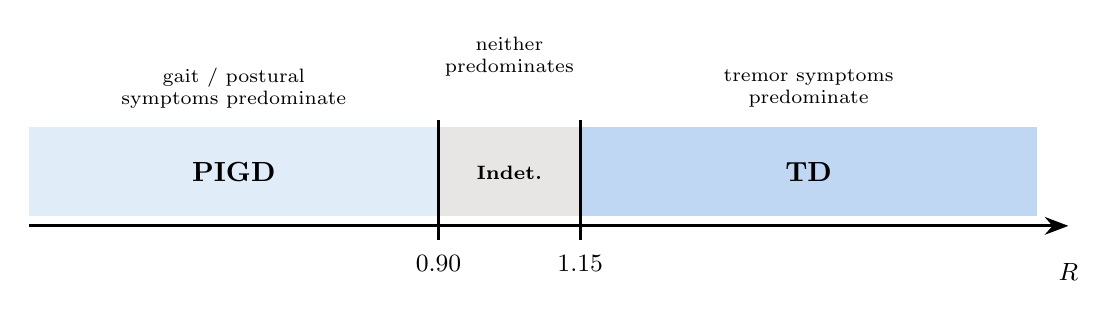
\begin{tikzpicture}[scale=1.0]
  % axis
  \draw[line width=1pt,-{Stealth[length=3mm]}] (0,0) -- (13.2,0);
  \node[below] at (13.2,-0.35) {\small $R$};

  % bands
  \fill[accent!14] (0,0.12) rectangle (5.2,1.25);
  \fill[rule!45]   (5.2,0.12) rectangle (7.0,1.25);
  \fill[accent!30] (7.0,0.12) rectangle (12.8,1.25);

  \draw[line width=1pt] (5.2,-0.18) -- (5.2,1.35);
  \draw[line width=1pt] (7.0,-0.18) -- (7.0,1.35);

  \node[below] at (5.2,-0.25) {\small $0.90$};
  \node[below] at (7.0,-0.25) {\small $1.15$};

  \node at (2.6,0.68) {\textbf{PIGD}};
  \node at (6.1,0.68) {\scriptsize\textbf{Indet.}};
  \node at (9.9,0.68) {\textbf{TD}};

  \node[align=center,font=\scriptsize] at (2.6,1.75)
        {gait / postural\\symptoms predominate};
  \node[align=center,font=\scriptsize] at (6.1,2.15) {neither\\predominates};
  \node[align=center,font=\scriptsize] at (9.9,1.75)
        {tremor symptoms\\predominate};
\end{tikzpicture}
\caption{The classification rule as a single axis. \textbf{What to notice:} the
Indeterminate band occupies only $0.25$ units of a scale on which observed
values range from $0$ to over $11$. Section~\ref{sec:noise} shows that this
narrowness has consequences.}
\label{fig:rule}
\end{figure}

\subsection{Problem statement}

The rule above describes a patient at a \emph{single} visit. It answers the
question:

\begin{center}
\emph{``What subtype does this patient appear to have today?''}
\end{center}

Parkinson's disease, however, progresses over time, and a patient's recorded
subtype can differ from one visit to the next. This raises a question the
existing rule cannot answer:

\begin{center}
\emph{``How does the subtype change over time, and how confident can we be that
an observed change represents genuine progression?''}
\end{center}

An observed change from TD to PIGD may reflect real disease progression. It may
equally reflect ordinary variability in a clinical examination --- a slightly
different rating on one item, on one day, by one examiner. Distinguishing these
two possibilities is the central problem this project addresses.

\subsection{Project objective}

\begin{keypoint}
\textbf{The objective of this project is to develop a probabilistic
understanding of motor subtype progression using longitudinal PPMI data.}
\end{keypoint}

\noindent
This breaks into three concrete aims:

\begin{enumerate}
  \item Build a reliable longitudinal dataset in which each visit carries a
        trustworthy subtype label.
  \item Establish what the data actually shows about how those labels change
        over time.
  \item Develop models that distinguish genuine progression from variability in
        the observed labels.
\end{enumerate}

\subsection{Research questions}

\begin{enumerate}
  \item How frequently does the recorded motor subtype change between visits,
        and in which directions?
  \item Is the Indeterminate category a stable subtype or a transitional
        region?
  \item Can the observed sequence of subtypes be described by a model that uses
        only the current label, or is a richer description required?
  \item Once measurement variability is accounted for, how stable is a
        patient's underlying motor state?
  \item Does the continuous TD/PIGD ratio show a systematic population-level
        trend, and at what rate?
\end{enumerate}

\subsection{How the project developed}

Each stage of this project was motivated by what the previous stage revealed.
The report follows that sequence rather than the order in which the software was
written.

\begin{figure}[H]
\centering
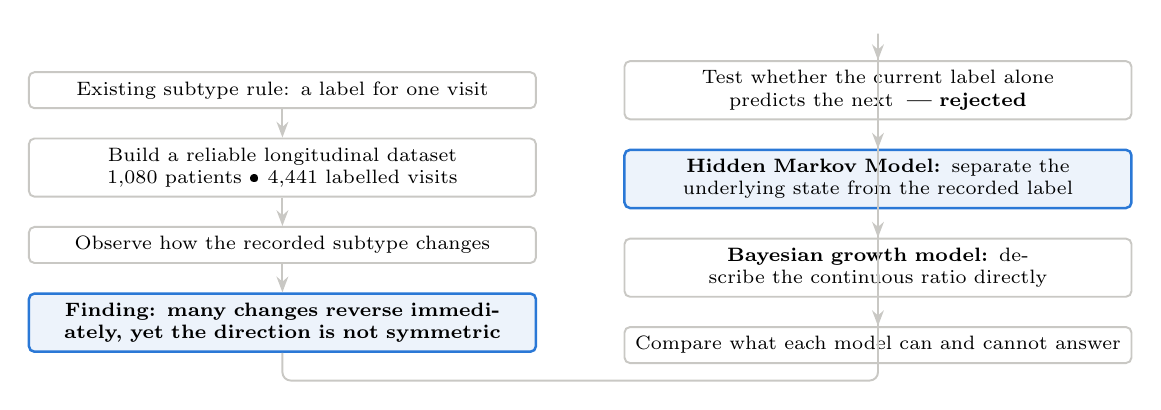
\begin{tikzpicture}[
    node distance=3.6mm,
    box/.style={draw=rule,line width=0.7pt,rounded corners=2pt,fill=white,
                text width=6.2cm,align=center,inner sep=3.4pt,font=\scriptsize},
    hl/.style={box,fill=soft,draw=accent,line width=0.9pt},
    ar/.style={-{Stealth[length=2mm]},line width=0.7pt,draw=rule}]

  \node[box]              (a) {Existing subtype rule: a label for one visit};
  \node[box,below=of a]   (b) {Build a reliable longitudinal dataset\\
                               1,080 patients \textbullet\ 4,441 labelled visits};
  \node[box,below=of b]   (c) {Observe how the recorded subtype changes};
  \node[hl,below=of c]    (d) {\textbf{Finding: many changes reverse immediately,
                               yet the direction is not symmetric}};
  \draw[ar] (a)--(b); \draw[ar] (b)--(c); \draw[ar] (c)--(d);

  \node[box,right=11mm of a] (e) {Test whether the current label alone predicts
                                  the next \;\textbf{--- rejected}};
  \node[hl,below=of e]       (f) {\textbf{Hidden Markov Model:} separate the
                                  underlying state from the recorded label};
  \node[box,below=of f]      (g) {\textbf{Bayesian growth model:} describe the
                                  continuous ratio directly};
  \node[box,below=of g]      (h) {Compare what each model can and cannot answer};
  \draw[ar] (e)--(f); \draw[ar] (f)--(g); \draw[ar] (g)--(h);

  \draw[ar,rounded corners=3pt] (d.south) -- ++(0,-3.5mm)
        -| ($(e.north)+(0,4mm)$) -- (e.north);
\end{tikzpicture}
\caption{The logic of the project. \textbf{What to notice:} the two shaded boxes
are the points at which a finding in the data forced a change of method. Neither
model was chosen in advance.}
\label{fig:workflow}
\end{figure}

% =============================================================================
\section{Data and Motor Subtype Classification}
% =============================================================================

\subsection{The PPMI dataset}

The Parkinson's Progression Markers Initiative (PPMI) is a large international
observational study that follows Parkinson's disease patients over many years,
recording a standardised clinical assessment at each visit. It is well suited to
this project because the same examination is repeated on the same patients over
long periods, which is exactly what is needed to observe how a subtype changes.

We used three components: the Curated Data Cut, which provides the visit
structure and patient characteristics; the item-level MDS-UPDRS Part II and
Part III files, which provide the sixteen individual scores from which the
subtype is computed; and an archived data release, used only to check our work.

\subsection{Why the classification was recomputed}

PPMI publishes a subtype variable of its own, so a natural question is why we
did not simply use it. There were two reasons. First, the published variable in
the Curated Data Cut is effectively two-class and does not preserve the
Indeterminate category, which --- as Section~\ref{sec:indet} shows --- turns out
to be central to the findings. Second, it does not publish the underlying tremor
and gait subscores, and therefore not the continuous ratio, which the model in
Chapter~\ref{sec:bayes} requires.

We therefore recomputed the classification from the individual item scores. This
also made it possible to verify the result against PPMI's own labels, which is
reported in Section~\ref{sec:validation}.

\subsection{Constructing the longitudinal dataset}

\begin{figure}[H]
\centering
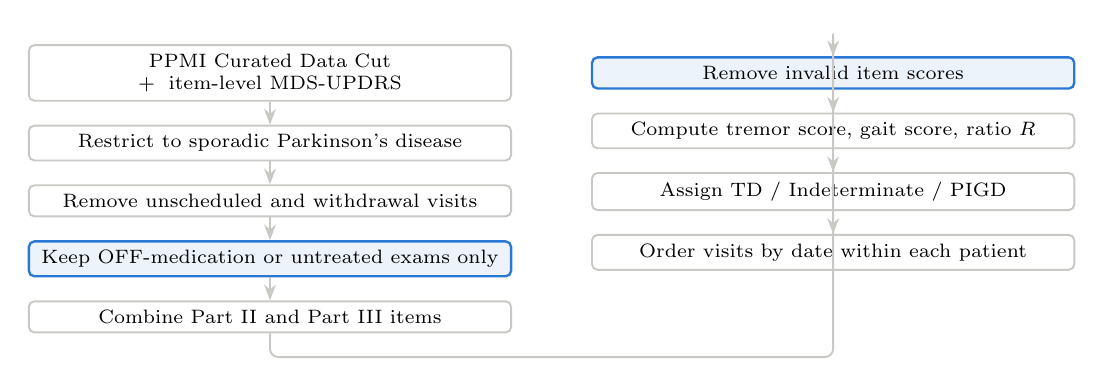
\begin{tikzpicture}[
    node distance=2.9mm,
    st/.style={draw=rule,line width=0.7pt,rounded corners=2pt,fill=white,
               text width=5.9cm,align=center,inner sep=3.2pt,font=\scriptsize},
    hl/.style={st,fill=soft,draw=accent,line width=0.85pt},
    ar/.style={-{Stealth[length=2mm]},line width=0.7pt,draw=rule}]

  \node[st]             (s1) {PPMI Curated Data Cut \;+\; item-level MDS-UPDRS};
  \node[st,below=of s1] (s2) {Restrict to sporadic Parkinson's disease};
  \node[st,below=of s2] (s3) {Remove unscheduled and withdrawal visits};
  \node[hl,below=of s3] (s4) {Keep OFF-medication or untreated exams only};
  \node[st,below=of s4] (s5) {Combine Part II and Part III items};
  \draw[ar](s1)--(s2);\draw[ar](s2)--(s3);\draw[ar](s3)--(s4);\draw[ar](s4)--(s5);

  \node[hl,right=10mm of s1] (s6) {Remove invalid item scores};
  \node[st,below=of s6]      (s7) {Compute tremor score, gait score, ratio $R$};
  \node[st,below=of s7]      (s8) {Assign TD / Indeterminate / PIGD};
  \node[st,below=of s8]      (s9) {Order visits by date within each patient};
  \draw[ar](s6)--(s7);\draw[ar](s7)--(s8);\draw[ar](s8)--(s9);

  \draw[ar,rounded corners=3pt] (s5.south) -- ++(0,-3mm)
        -| ($(s6.north)+(0,3.5mm)$) -- (s6.north);
\end{tikzpicture}
\caption{Construction of the longitudinal dataset. \textbf{What to notice:} two
of these steps --- the medication filter and the removal of invalid scores ---
change the resulting labels substantially and are explained in
Section~\ref{sec:quality}.}
\label{fig:pipeline}
\end{figure}

\noindent
Two aspects of the construction are worth stating explicitly.

\paragraph{Only sporadic Parkinson's disease was included.}
PPMI also follows patients carrying specific genetic mutations. Those forms of
the disease are believed to progress differently, so including them would mix
genetic effects into the progression estimates. Restricting to sporadic disease
keeps the population homogeneous.

\paragraph{Time was measured from actual visit dates.}
PPMI labels visits by nominal year, but patients do not attend on schedule. All
intervals in this report are computed from recorded visit dates, because the
gap between two visits turns out to matter (Section~\ref{sec:interval}).

\subsection{Data cleaning and two quality issues}
\label{sec:quality}

Two issues in the raw data affect the resulting classification enough to be
worth describing.

\paragraph{Invalid score values.}
The valid range for an MDS-UPDRS item is $0$ to $4$. However, PPMI records the
value $101$ to mean \emph{``Unable to Rate''} --- for instance when a patient
cannot safely be tested for postural stability --- and it is stored in the same
numeric field as a real score. Treated as a score, a single such value among the
five gait items raises their average to roughly $20$, which drives the ratio
close to zero and misclassifies a clearly tremor-dominant visit as PIGD. These
values were therefore excluded before any score was computed. This is not a rare
edge case: the postural-stability item alone carries 4{,}302 of them.

\paragraph{Medication state.}
Parkinson's medication suppresses tremor considerably more than it improves gait
and balance. An examination performed while a patient is medicated therefore
lowers the numerator of the ratio while leaving the denominator largely intact,
pushing the patient towards a PIGD classification for reasons that have nothing
to do with disease progression. We therefore used only OFF-medication or
untreated examinations, which is also what the original definition of the
classification specifies. Note that this filters \emph{examinations}, not
patients: a medicated patient still contributes through their OFF assessment.

\subsection{Validation of the classification}
\label{sec:validation}

Because the classification was recomputed rather than taken from the database,
it had to be checked. We compared our labels against PPMI's own on the visits
where both exist.

\begin{table}[H]
\centering
\begin{tabular}{@{}lcr@{}}
\toprule
\textbf{Reference} & \textbf{Comparison} & \textbf{Agreement} \\
\midrule
PPMI Curated Data Cut          & two-class (TD vs.\ PIGD)              & 100.00\% \\
Archived PPMI data release     & three-class (incl.\ Indeterminate)    & \phantom{0}99.87\% \\
\bottomrule
\end{tabular}
\caption{Agreement between our recomputed labels and PPMI's own.}
\end{table}

\noindent
Two comparisons are reported because they test different things. The curated
variable is two-class, so agreement with it confirms that the tremor and gait
subscores and the main threshold are computed correctly, but says nothing about
the Indeterminate band. The archived release is the only source in the dataset
carrying a three-class label, so it is the only available check on the
Indeterminate boundary. Agreement of 99.87\% there --- the remaining
disagreements being visits whose ratio falls essentially exactly on a threshold
--- establishes that our labels reproduce PPMI's across all three categories.

\subsection{The final dataset}

\begin{table}[H]
\centering
\begin{tabular}{@{}lr@{}}
\toprule
\textbf{Quantity} & \textbf{Value} \\
\midrule
Patients                                        & 1{,}080 \\
Visits                                          & 5{,}774 \\
Visits with a valid subtype label               & 4{,}441 \;(76.9\%) \\
Consecutive labelled visit pairs (transitions)  & 3{,}361 \\
Patients contributing at least one transition   & \phantom{0,}934 \\
Median interval between visits                  & 1.0 year \\
Median labelled visits per patient              & 3 \;(maximum 14) \\
Maximum follow-up                               & 14.0 years \\
\midrule
Subtype distribution, all labelled visits       & TD 65.1\% \textbullet\ Indet.\ 9.9\% \textbullet\ PIGD 25.0\% \\
Subtype distribution at the first visit         & TD 71.7\% \textbullet\ Indet.\ 10.1\% \textbullet\ PIGD 18.1\% \\
\bottomrule
\end{tabular}
\caption{The dataset used throughout this report.}
\end{table}

\noindent
The comparison between the last two rows is already informative: the proportion
of PIGD visits is higher across all visits (25.0\%) than at the first visit
(18.1\%), which is a first indication of net movement towards PIGD over time.

% =============================================================================
\section{Observed Motor Subtype Progression}
% =============================================================================

This chapter reports what the data shows before any model is introduced. The
findings here are the ones that determined which models were subsequently used.

\subsection{Visit-to-visit transitions}

For each of the 3{,}361 consecutive pairs of labelled visits we recorded the
subtype at both ends. Expressed as proportions of each starting state:

\begin{table}[H]
\centering
\begin{tabular}{@{}lccc@{}}
\toprule
\textbf{Current visit} & \textbf{$\rightarrow$ TD} & \textbf{$\rightarrow$ Indeterminate} & \textbf{$\rightarrow$ PIGD} \\
\midrule
TD             & \textbf{80.8\%} & 8.0\%           & 11.2\% \\
Indeterminate  & 44.0\%          & \textbf{19.2\%} & 36.8\% \\
PIGD           & 18.4\%          & 11.4\%          & \textbf{70.2\%} \\
\bottomrule
\end{tabular}
\caption{Observed transition probabilities. Rows sum to 100\%.}
\end{table}

\begin{figure}[H]
\centering
\includegraphics[width=0.50\textwidth]{transition_matrix.png}
\caption{The same information as a heatmap. \textbf{What to notice:} the
diagonal is dark for TD and PIGD but light for Indeterminate, and the
off-diagonal cells in the Indeterminate row are the largest in the table.}
\end{figure}

\subsection{Indeterminate behaves as a transitional region}
\label{sec:indet}

\begin{keypoint}
\textbf{Finding 1. Indeterminate is not a stable subtype.} Only \textbf{19.2\%}
of visits classified as Indeterminate are followed by another Indeterminate
visit. The remaining 80.8\% move to TD (44.0\%) or PIGD (36.8\%).
\end{keypoint}

\noindent
By contrast, TD persists in 80.8\% of cases and PIGD in 70.2\%. Indeterminate is
therefore behaving less like a third subtype and more like a boundary region
that patients pass through. This has a direct consequence for modelling: any
model that treats the three categories as three comparable states will
misrepresent the middle one.

\subsection{PIGD is not a one-way destination}

A common expectation is that patients progress from TD towards PIGD and remain
there. The data does not support the second half of that expectation.

\begin{keypoint}
\textbf{Finding 2. PIGD is not absorbing.} \textbf{29.8\%} of PIGD visits are
followed by a non-PIGD classification, and \textbf{18.4\%} are followed directly
by TD.
\end{keypoint}

\noindent
This should be interpreted carefully. It does not mean that Parkinson's disease
reverses. The more plausible reading is that the \emph{recorded} subtype is
affected by variability in the examination, so that some patients recorded as
PIGD at one visit were not in fact predominantly PIGD. That interpretation is
tested directly in the next section.

\begin{figure}[H]
\centering
\includegraphics[width=0.80\textwidth]{pathway_flow.png}
\caption{Subtype pathways followed by individual patients over the whole
follow-up period, with repeated states collapsed so that only changes are shown.
\textbf{What to notice:} very few patients follow a single clean transition.
Most pathways that reach PIGD pass through Indeterminate, and many return.}
\end{figure}

\subsection{Many observed changes reverse immediately}
\label{sec:noise}

If a change from one subtype to another reflects genuine progression, we would
not expect it to be undone at the very next visit. We therefore took every
observed change and asked what happened next.

\begin{keypoint}
\textbf{Finding 3. \textbf{35.2\%} of observed subtype changes reverse at the
following visit} --- the patient returns to the subtype they held before the
change.
\end{keypoint}

\begin{figure}[H]
\centering
\includegraphics[width=0.62\textwidth]{reversion.png}
\caption{Proportion of changes reversed at the next visit, by type of change.
\textbf{What to notice:} the rate is not uniform.}
\end{figure}

\noindent
The breakdown by direction is more informative than the overall figure:

\begin{table}[H]
\centering
\begin{tabular}{@{}lrr@{}}
\toprule
\textbf{Observed change} & \textbf{Number} & \textbf{Reversed next visit} \\
\midrule
TD $\rightarrow$ Indeterminate   & 134 & \textbf{56.0\%} \\
PIGD $\rightarrow$ Indeterminate & \phantom{0}54 & \textbf{50.0\%} \\
PIGD $\rightarrow$ TD            & 112 & 39.3\% \\
TD $\rightarrow$ PIGD            & 172 & 32.0\% \\
Indeterminate $\rightarrow$ PIGD & \phantom{0}93 & 18.3\% \\
Indeterminate $\rightarrow$ TD   & 108 & \textbf{17.6\%} \\
\bottomrule
\end{tabular}
\caption{Reversal rate by type of change. Only changes followed by a further
visit can be assessed, giving 673 assessable changes.}
\end{table}

\noindent
Movements \emph{into} Indeterminate reverse about half the time; movements
\emph{out of} Indeterminate reverse less than a fifth of the time. This is what
one would expect if Indeterminate is a narrow band that patients momentarily
appear to occupy because of ordinary measurement variation, rather than a state
they genuinely enter and leave. It reinforces Finding~1 from an independent
direction.

\subsection{But the changes are not merely random}

Reversal alone might suggest that observed changes carry no information. The
direction of movement shows otherwise.

\begin{keypoint}
\textbf{Finding 4. Movement is directionally biased towards PIGD.} Over the
whole dataset there were \textbf{253} changes from TD to PIGD against
\textbf{141} from PIGD to TD ($p = 1.8 \times 10^{-8}$).
\end{keypoint}

\noindent
If observed changes were purely random measurement fluctuations, movement in one
direction would be balanced by movement in the other. It is not. Taken together,
Findings~3 and~4 give the central conclusion of this chapter:

\begin{keypoint}
The data is consistent with \textbf{two effects operating simultaneously}: a
genuine, gradual, directional progression towards PIGD, \emph{observed through a
measurement that carries substantial variability}. Any adequate model must
represent both.
\end{keypoint}

\subsection{The interval between visits matters}
\label{sec:interval}

Patients do not attend at regular intervals. We therefore recomputed the
transition table separately for short and long gaps between visits.

\begin{figure}[H]
\centering
\includegraphics[width=0.76\textwidth]{transitions_by_interval.png}
\caption{Transition probabilities stratified by the elapsed interval between the
two visits. \textbf{What to notice:} the probability of leaving the current
subtype increases as the gap grows.}
\end{figure}

\noindent
A patient reassessed after four years has had far more time in which to change
than one reassessed after six months. Treating every visit-to-visit transition
as though it spanned the same amount of time is therefore inappropriate, and any
model must take the elapsed interval as an input rather than ignoring it.

\subsection{Time to PIGD conversion}

A natural clinical question is how long it takes for a patient to convert to
PIGD. Answering it requires care, because patients have very unequal follow-up:
some contributed two visits and some fourteen. Simply reporting the percentage
who ever converted would treat those patients as equivalent. We therefore used
survival analysis, which accounts properly for patients whose follow-up ends
before any conversion is seen.

\begin{table}[H]
\centering
\begin{tabular}{@{}lrrr@{}}
\toprule
\textbf{Definition of conversion} & \textbf{At risk} & \textbf{Converted} & \textbf{5-year incidence} \\
\midrule
Any single PIGD visit              & 885 & 263 & 35.3\% \\
PIGD sustained over two visits     & 885 & 127 & 15.3\% \\
\bottomrule
\end{tabular}
\caption{Estimated cumulative incidence of PIGD conversion under two
definitions.}
\end{table}

\begin{figure}[H]
\centering
\includegraphics[width=0.58\textwidth]{time_to_pigd_conversion.png}
\caption{Estimated proportion of patients yet to convert to PIGD, under both
definitions. \textbf{What to notice:} the two curves separate widely, and the
confidence bands broaden at the right-hand end where few patients remain under
observation.}
\end{figure}

\noindent
The gap between the two rows is itself a finding. Requiring that a PIGD
classification persist across two consecutive visits --- rather than accepting a
single one --- more than halves the estimated five-year conversion rate, from
35.3\% to 15.3\%. Much of the apparent conversion under the looser definition
consists of single PIGD visits that are not repeated, which is exactly the
pattern described in Section~\ref{sec:noise}. Reported conversion rates for this
subtype are therefore highly sensitive to a definitional choice that is not
always made explicit.

\subsection{A limitation with a known direction}

\begin{caveat}{Important limitation: missing data is not random}
A visit can only be assigned a subtype if all sixteen required MDS-UPDRS items
were recorded. This was not the case for \textbf{23.1\%} of visits in the
cohort.

Crucially, the missingness is not random. Items go unrecorded most often when a
patient cannot complete the assessment --- postural stability being the clearest
example --- and this occurs more frequently in patients with more advanced
disease. Because more advanced patients are also more likely to be PIGD, the
visits excluded from this analysis are disproportionately those that would have
been classified as PIGD.

\vspace{4pt}
\textbf{Consequence:} the progression rates reported throughout this report
should be interpreted as \textbf{lower bounds}. The true rate of movement
towards PIGD is likely to be somewhat higher than estimated here.
\end{caveat}

% =============================================================================
\section{Probabilistic Modelling of Progression}
% =============================================================================

\subsection{The modelling problem}

Chapter~3 established that a subtype change may reflect genuine progression or
examination variability, and that both are present in the data. The modelling
task is therefore:

\begin{center}
\emph{Given a patient's sequence of recorded subtypes and the times at which
they were recorded, describe how their motor state is progressing.}
\end{center}

We approached this by testing progressively richer descriptions, beginning with
the simplest one that could plausibly work.

\subsection{Why a simple model is not sufficient}

The simplest description of a sequence of states assumes that the current state
contains all the information needed to predict the next one --- that once you
know a patient is TD today, knowing what they were two years ago tells you
nothing more. This is the \emph{Markov assumption}, and it underlies the
standard approach to modelling categorical progression.

We tested it directly, using every sequence of three consecutive labelled visits
and asking whether the visit before last changes the prediction.

\begin{keypoint}
\textbf{The assumption is rejected}, and decisively: $\chi^2 = 156.6$,
$p = 7.9 \times 10^{-33}$.
\end{keypoint}

\noindent
The size of the effect matters as much as its significance. Consider only
patients whose current visit is recorded as TD:

\begin{table}[H]
\centering
\begin{tabular}{@{}lccc@{}}
\toprule
\textbf{Previous visit} & \textbf{$\rightarrow$ TD} & \textbf{$\rightarrow$ Indeterminate} & \textbf{$\rightarrow$ PIGD} \\
\midrule
TD             & 84.9\% & \phantom{0}6.5\% & \phantom{0}\textbf{8.6\%} \\
Indeterminate  & 52.8\% & 17.6\%           & 29.6\% \\
PIGD           & 48.2\% & 12.5\%           & \textbf{39.3\%} \\
\bottomrule
\end{tabular}
\caption{Where patients currently recorded as TD go next, according to where
they came from.}
\end{table}

\noindent
A patient recorded as TD today has an 8.6\% chance of being recorded PIGD next
visit if they were also TD last time --- but a 39.3\% chance if they were PIGD
last time. The current label plainly does not contain everything relevant.

This is not merely a negative result. A process in which history predicts the
future in exactly this way is the characteristic signature of a system in which
the \emph{observed} label is an imperfect reading of some underlying state. The
failed test therefore indicates which kind of model is needed.

\subsection{Separating the underlying state from the recorded label}

\begin{figure}[H]
\centering
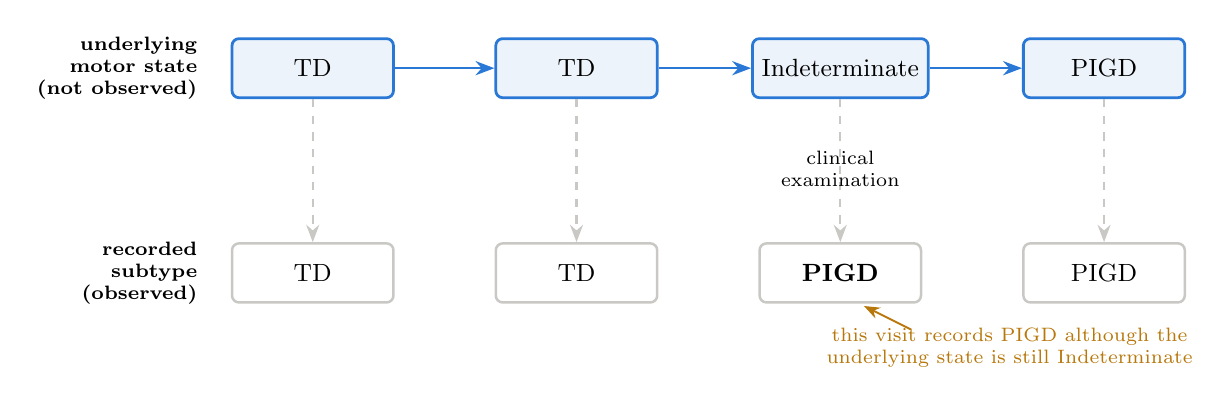
\begin{tikzpicture}[
    st/.style={draw=accent,line width=1pt,rounded corners=2.5pt,fill=soft,
               minimum width=2.05cm,minimum height=0.75cm,font=\small},
    ob/.style={draw=rule,line width=0.9pt,rounded corners=2.5pt,fill=white,
               minimum width=2.05cm,minimum height=0.75cm,font=\small},
    tr/.style={-{Stealth[length=2.4mm]},line width=0.9pt,draw=accent},
    em/.style={-{Stealth[length=2.2mm]},line width=0.8pt,draw=rule,dashed}]

  \node[st] (u1) at (0,2.6)    {TD};
  \node[st] (u2) at (3.35,2.6) {TD};
  \node[st] (u3) at (6.7,2.6)  {Indeterminate};
  \node[st] (u4) at (10.05,2.6){PIGD};

  \node[ob] (o1) at (0,0)    {TD};
  \node[ob] (o2) at (3.35,0) {TD};
  \node[ob] (o3) at (6.7,0)  {\textbf{PIGD}};
  \node[ob] (o4) at (10.05,0){PIGD};

  \draw[tr] (u1)--(u2); \draw[tr] (u2)--(u3); \draw[tr] (u3)--(u4);
  \draw[em] (u1)--(o1); \draw[em] (u2)--(o2);
  \draw[em] (u3)--(o3); \draw[em] (u4)--(o4);

  \node[left=3mm of u1,align=right,font=\scriptsize\bfseries]
       {underlying\\motor state\\(not observed)};
  \node[left=3mm of o1,align=right,font=\scriptsize\bfseries]
       {recorded\\subtype\\(observed)};

  \node[font=\scriptsize,align=center] at (6.7,1.32)
       {clinical\\examination};
  \node[font=\scriptsize,align=center,text=warn] at (8.85,-0.95)
       {this visit records PIGD although the\\
        underlying state is still Indeterminate};
  \draw[-{Stealth[length=2mm]},line width=0.7pt,draw=warn]
       (7.6,-0.72) -- (7.0,-0.42);
\end{tikzpicture}
\caption{The idea behind the Hidden Markov Model. \textbf{What to notice:} the
top row progresses smoothly and in one direction; the bottom row --- which is
all we actually see --- appears to jump. The model's task is to infer the top
row from the bottom row.}
\label{fig:hmm}
\end{figure}

\noindent
The model we used makes the distinction in Figure~\ref{fig:hmm} explicit. It
supposes that each patient has an underlying motor state which changes gradually
over time, and that each clinical examination produces a recorded subtype which
usually --- but not always --- matches it. The model estimates two things at
once from the data: how quickly underlying states change, and how reliably each
one is recorded.

This is implemented as a \textbf{Hidden Markov Model} (HMM). ``Hidden'' refers to
the underlying state, which is never observed directly. Because the intervals
between visits are irregular (Section~\ref{sec:interval}), the underlying state
is modelled as changing in continuous time, so the elapsed gap between two
visits enters the model directly.

For comparison we also fitted three simpler models: a Markov chain applied to
the observed labels; the same chain made interval-aware; and a null model that
ignores the current state entirely and predicts the overall subtype
distribution. The null model exists to establish a floor --- any model that
cannot beat it is not using the information available.

\subsection{Model validation}

All models were compared on patients whose data was withheld during fitting. The
split was made \emph{by patient}, not by visit: every visit belonging to a given
patient was assigned entirely to either the training or the test set. Splitting
by visit would allow the same patient to appear on both sides and would make the
models look better than they are.

\begin{table}[H]
\centering
\begin{tabular}{@{}lrr@{}}
\toprule
\textbf{Model} & \textbf{Accuracy} & \textbf{Brier score} \\
\midrule
Hidden Markov Model                & \textbf{76.9\%} & \textbf{0.346} \\
Markov chain on observed labels    & 76.7\%          & 0.363 \\
Interval-aware Markov chain        & 76.5\%          & 0.367 \\
Null model (no use of state)       & 62.5\%          & 0.519 \\
\bottomrule
\end{tabular}
\caption{Performance on 1{,}002 held-out transitions from patients not used in
fitting. Brier score measures the quality of the predicted probabilities, and
lower is better; accuracy alone rewards only the single most likely prediction.}
\end{table}

\noindent
Accuracy separates the models only slightly, because all of them get the easy
cases right --- a TD patient usually remains TD. The Brier score separates them
more clearly, because it evaluates the whole predicted probability distribution
rather than only the most likely outcome. This is the more relevant measure for
a model intended to express uncertainty.

\begin{keypoint}
The Hidden Markov Model outperformed the plain Markov chain in \textbf{all ten}
independent splits, by an average margin of $0.028$ in held-out log-likelihood
per transition (standard deviation $0.009$). The improvement is small but
entirely consistent.
\end{keypoint}

\subsection{What the model tells us}

The model's predictive advantage is modest. Its interpretative value is larger,
because the quantities it estimates answer questions the raw transition table
cannot.

\paragraph{Finding 5: progression is mostly sequential.}
The estimated rates of change between underlying states are:
\[
  \text{TD} \rightarrow \text{Indeterminate}: \; 0.094 \text{ per year}
  \qquad
  \text{TD} \rightarrow \text{PIGD}: \; 0.006 \text{ per year}
\]
Movement from TD directly to PIGD is estimated to be roughly sixteen times rarer
than movement from TD into Indeterminate. The model therefore describes
progression as passing \emph{through} the intermediate region rather than
jumping across it --- consistent with the pathway structure seen in
Section~\ref{sec:indet}, and reached here by an entirely separate route.

\paragraph{Finding 6: the recorded label is much less reliable for Indeterminate.}
The model estimates, for each underlying state, how often an examination records
it correctly:

\begin{table}[H]
\centering
\begin{tabular}{@{}lc@{}}
\toprule
\textbf{Underlying state} & \textbf{Recorded correctly} \\
\midrule
TD             & 94.1\% \\
PIGD           & 84.2\% \\
Indeterminate  & \textbf{50.0\%} \\
\bottomrule
\end{tabular}
\caption{Estimated probability that an examination records the underlying state
correctly.}
\end{table}

\begin{figure}[H]
\centering
\includegraphics[width=0.52\textwidth]{misclassification.png}
\caption{Estimated relationship between underlying state and recorded label.
\textbf{What to notice:} the TD and PIGD rows are concentrated on the diagonal;
the Indeterminate row is spread across all three columns.}
\end{figure}

\noindent
TD and PIGD are recorded reliably. Indeterminate is recorded correctly only
about half the time. This is a third independent line of evidence pointing at
the same conclusion as Findings~1 and~3, and there is a simple explanation for
it: the Indeterminate band is only $0.25$ units wide (Figure~\ref{fig:rule}),
which is small relative to the variation observed in the ratio between
consecutive visits of the same patient.

\paragraph{Finding 7: underlying states are more stable than the labels suggest.}
Once measurement variability is accounted for, the model estimates how long a
patient remains in an underlying state before genuinely moving on:

\begin{table}[H]
\centering
\begin{tabular}{@{}lrr@{}}
\toprule
\textbf{State} & \textbf{From observed labels} & \textbf{Estimated underlying state} \\
\midrule
TD             & 3.4 years & \textbf{10.1 years} \\
Indeterminate  & 0.4 years & \phantom{0}\textbf{2.1 years} \\
PIGD           & 2.3 years & \textbf{16.5 years} \\
\bottomrule
\end{tabular}
\caption{Estimated persistence of a motor state, before and after accounting for
variability in the examination.}
\end{table}

\begin{figure}[H]
\centering
\includegraphics[width=0.60\textwidth]{sojourn_comparison.png}
\caption{Persistence of each motor state as read from the observed labels
against the model's estimate for the underlying state. \textbf{What to notice:}
the gap is large for every state, and largest for PIGD.}
\end{figure}

\begin{keypoint}
\textbf{The underlying motor state appears to be roughly three to seven times
more persistent than the recorded subtype suggests.} On this reading, most of
the apparent instability seen in Chapter~3 is variability in the examination
rather than genuine change in the patient.
\end{keypoint}

\noindent
This is the most substantial claim in the report, and it should be read as the
model's interpretation of the data rather than as a directly measured quantity.
Its plausibility rests on the fact that three independent analyses --- the
persistence of Indeterminate, the pattern of immediate reversals, and the
estimated reliability of the recording --- all point the same way.

% =============================================================================
\section{A Bayesian Model of the TD/PIGD Ratio}
\label{sec:bayes}
% =============================================================================

\subsection{Why a second model}

The model in Chapter~4 works with the three discrete subtypes. But the
classification is derived from a continuous quantity --- the ratio $R$ --- and
converting it into three categories discards information. A patient whose ratio
falls from $4.0$ to $2.0$ has changed considerably, yet remains TD throughout
and contributes nothing to a transition-based analysis.

We therefore asked a different question:

\begin{center}
\emph{``Does the ratio itself show a systematic trend over time, and how fast?''}
\end{center}

\noindent
This is a question about \emph{rate}, which the discrete model cannot answer at
all. It was also the modelling approach suggested in the original project
proposal.

\subsection{The idea of the model}

The model describes each patient's ratio as following its own straight line over
time:

\[
  R_{it} \;=\; \underbrace{\text{patient's starting level}}_{\text{differs between patients}}
  \;+\; \underbrace{\text{patient's rate of change}}_{\text{differs between patients}} \times t
  \;+\; \underbrace{\text{variation}}_{\text{differs between visits}}
\]

Three ideas are combined here. Each patient has their own starting level and
their own rate. Those individual values are not free to be anything: the model
assumes they are drawn from a population distribution, so that a patient with
few visits is described mostly by the population average and a patient with many
visits is allowed to depart from it. And each individual measurement is allowed
to deviate from the patient's own line.

This structure is called a \textbf{hierarchical Bayesian growth model}. The
``hierarchical'' part is the assumption that individual patients come from a
common population; the ``Bayesian'' part means the result is not a single
estimate but a distribution expressing how certain we are about each quantity.

Four quantities are estimated: the population starting level, the population
rate of change, how much patients differ from one another, and how much
individual visits vary around a patient's own line.

\subsection{The population progression rate}

\begin{center}
\fcolorbox{accent}{soft}{%
\begin{minipage}{0.86\textwidth}
\vspace{4pt}
\centering
\textbf{Estimated population progression rate}
\[
  \beta_1 \;=\; -0.0927 \text{ per year}
  \qquad
  \text{95\% credible interval } [-0.1159,\; -0.0682]
\]
\vspace{-6pt}
\end{minipage}}
\end{center}

\vspace{6pt}
\noindent
The TD/PIGD ratio declines by approximately $0.093$ per year on average. The
estimated probability that the population rate is negative --- that is, that the
population as a whole is drifting towards PIGD --- is essentially 100\%.

A ``credible interval'' can be read in the natural way: given the model and the
data, there is a 95\% probability that the population rate lies between $0.068$
and $0.116$ per year.

To put the rate in context: from the estimated population starting level of
$2.29$, an average trajectory takes approximately \textbf{12.3 years} to fall to
the TD threshold of $1.15$. Progression at the population level is therefore a
slow drift measured in decades, not a rapid conversion.

\subsection{Variation between patients}

\begin{figure}[H]
\centering
\includegraphics[width=0.94\textwidth]{growth_trajectories.png}
\caption{Left: the estimated population trajectory with individual variation.
Right: the estimated progression rate.}
\label{fig:growth}
\end{figure}

\noindent
Figure~\ref{fig:growth} requires explanation, because the two panels show
different kinds of quantity and are easily confused.

\paragraph{The blue line and band (left panel).}
The blue line is the estimated \emph{average} trajectory across the population.
The shaded band around it expresses how uncertain we are about that average. It
is narrow, because the estimate rests on thousands of observations.

\paragraph{The grey lines (left panel).}
The grey lines are \emph{example individual patients} generated from the
estimated variation between patients. They are not real patients, and they are
not intended to pass through any observed measurement. They illustrate the range
of individual trajectories that the fitted model considers plausible.

\paragraph{Why the grey lines are straight.}
Because the model describes each patient by a straight line, every trajectory
drawn from it is straight by construction. Real patients' measurements do not
lie on straight lines --- they vary considerably from visit to visit --- and
that variation is represented in the model by the third term of the equation,
which is simply not drawn in this figure. The figure shows modelled trends, not
observations.

\paragraph{The right panel.}
This shows the estimated population rate of change as a distribution rather than
a single number. The solid line marks the central estimate and the dotted lines
the bounds of the 95\% credible interval. The entire distribution lies well away
from zero, which is the visual form of the statement that the population is
progressing.

\paragraph{What the comparison shows.}
The essential point of the left panel is the contrast between the narrow blue
band and the wide grey fan. We know the population \emph{average} precisely, and
individual patients \emph{differ from it a great deal}. The estimated spread of
individual rates is wide enough that a minority of patients are drifting in the
opposite direction, towards TD. These are two different things, and only the
first is reduced by collecting more data; the second is genuine variation
between people.

\subsection{Two important limitations}

Implementing this model surfaced two limitations that are worth stating plainly,
because they bear on how the result should be used.

\paragraph{Two sources of variation cannot be separated.}
The model as originally specified distinguished variation arising from the
disease process itself from variation arising from measurement. With one
measurement per visit, these two cannot be estimated separately: they enter the
observed ratio in exactly the same way, so the data can determine their combined
size but not how it divides between them. We therefore report the combined
variation only. (In statistical terms, the two components are not
\emph{identifiable}.) This matters because a statement about the underlying
ratio ideally refers to the disease process alone.

\paragraph{The assumed distribution does not match the data.}
The model assumes each measurement varies symmetrically around the patient's
line, following a normal distribution. The ratio does not behave this way. It
cannot be negative; it is strongly skewed towards high values; and it is exactly
zero at 7.0\% of visits, in patients with no measurable tremor. A consequence is
that the model places \textbf{12.2\%} of its five-year predictions below zero,
which is impossible for a ratio of non-negative scores. The growth model should
therefore be read as a description of the average trend, not as a predictive
model for individual patients.

\subsection{Comparison with the Hidden Markov Model}

Both models were evaluated on the same held-out transitions --- restricted to
the 825 that both are able to score, since the growth model cannot be applied to
visits where the ratio is undefined.

\begin{table}[H]
\centering
\begin{tabular}{@{}lrr@{}}
\toprule
 & \textbf{Accuracy} & \textbf{Brier score} \\
\midrule
Hidden Markov Model            & \textbf{76.1\%} & \textbf{0.357} \\
Bayesian growth model          & 73.7\%          & 0.379 \\
\bottomrule
\end{tabular}
\caption{Performance on 825 shared held-out transitions. (These figures are not
directly comparable with the 76.9\% in Chapter~4, which was measured on the full
set of 1{,}002 held-out transitions.)}
\end{table}

\noindent
There is a measurable reason for the difference, and it is not a matter of one
model being better designed. The visit-to-visit variation in the ratio is
several times larger than the width of the Indeterminate band it must predict
membership of. Even a perfectly estimated trajectory therefore leaves the next
observation able to fall in any of the three categories. The discrete model
avoids this problem entirely by never attempting to predict a continuous value.

\begin{keypoint}
\textbf{The two models should not be read as competing attempts at the same
task.} The Hidden Markov Model is better suited to describing the sequence of
motor states and to separating the underlying state from the recorded label. The
Bayesian growth model is the only one of the two that provides an interpretable
rate of progression with a stated uncertainty.
\end{keypoint}

\begin{table}[H]
\centering
\begin{tabular}{@{}lll@{}}
\toprule
 & \textbf{Hidden Markov Model} & \textbf{Bayesian growth model} \\
\midrule
Question answered      & Which state is the patient in? & How fast is the ratio changing? \\
Works with             & Three discrete subtypes        & The continuous ratio \\
Handles noisy labels   & Yes, explicitly                & Only as combined variation \\
Gives a rate           & No                             & Yes, with an interval \\
Uses all visits        & Yes (4{,}441)                  & No (3{,}716) \\
Held-out accuracy      & 76.1\%                         & 73.7\% \\
\bottomrule
\end{tabular}
\caption{What each model is suited to.}
\end{table}

% =============================================================================
\section{Overall Findings}
% =============================================================================

\subsection{Summary of findings}

\begin{table}[H]
\centering
\small
\begin{tabular}{@{}p{7.9cm}p{7.9cm}@{}}
\toprule
\textbf{Finding} & \textbf{Evidence} \\
\midrule
The recorded subtype changes frequently &
19.2\% of TD, 80.8\% of Indeterminate and 29.8\% of PIGD visits are followed by
a different classification \\
\addlinespace
Indeterminate is a transitional region, not a stable subtype &
Only 19.2\% of Indeterminate visits are followed by another \\
\addlinespace
Many observed changes reverse immediately &
35.2\% overall, rising to 50--56\% for changes \emph{into} the Indeterminate
band \\
\addlinespace
The direction of change is nonetheless systematic &
253 changes TD $\rightarrow$ PIGD against 141 in the opposite direction
($p = 1.8\times10^{-8}$) \\
\addlinespace
The current label does not fully describe the patient's state &
Markov assumption rejected, $\chi^2 = 156.6$, $p = 7.9\times10^{-33}$; prior
state moves the probability of PIGD next visit from 8.6\% to 39.3\% \\
\addlinespace
Separating underlying state from recorded label describes the data better &
The Hidden Markov Model wins all ten independent validation splits \\
\addlinespace
Underlying states are more persistent than the labels suggest &
An estimated 10.1 years for TD and 16.5 for PIGD, against 3.4 and 2.3 as read
directly from the records \\
\addlinespace
The continuous ratio declines at the population level &
$0.093$ per year (95\% credible interval $0.068$--$0.116$), reaching the TD
threshold after approximately 12.3 years \\
\bottomrule
\end{tabular}
\end{table}

\subsection{Where the evidence converges}

The strongest conclusions are those supported by more than one independent
analysis.

\begin{table}[H]
\centering
\begin{tabular}{@{}p{6.0cm}p{8.2cm}@{}}
\toprule
\textbf{Conclusion} & \textbf{Independent lines of evidence} \\
\midrule
Indeterminate is a boundary region, not a subtype &
Persistence of only 19.2\%; reversal rate of 50--56\% for moves into it;
estimated recording reliability of 50.0\%; and progression modelled as passing
through it rather than around it \\
\addlinespace
The recorded label carries substantial noise &
35.2\% immediate reversal; failure of the Markov assumption; the gap between
observed and estimated underlying persistence; and the halving of the estimated
conversion rate when two consecutive visits are required \\
\addlinespace
Progression is genuine and directed towards PIGD &
Asymmetry of 253 against 141; the population ratio declining at 0.093 per year
with essentially 100\% posterior probability; and PIGD prevalence rising from
18.1\% at the first visit to 25.0\% across all visits \\
\bottomrule
\end{tabular}
\caption{Conclusions supported by multiple independent analyses.}
\end{table}

\subsection{What remains uncertain}

\begin{itemize}
  \item \textbf{How much of the observed instability is measurement variation.}
        The estimate that underlying states are three to seven times more
        persistent than the records suggest is a model-based inference. Its
        direction is well supported; its magnitude depends on the model.

  \item \textbf{Whether progression rates are constant over time.} All models
        here assume a constant rate. There is evidence in the data that the rate
        of movement towards PIGD is higher later in follow-up than earlier,
        which the current models do not represent.

  \item \textbf{Individual rates of progression.} The population rate is
        estimated precisely; an individual patient's rate is not. With a median
        of three visits per patient, an individual estimate is dominated by the
        population average rather than by that patient's own data.

  \item \textbf{Whether the findings hold outside PPMI.} No external cohort was
        used.
\end{itemize}

% =============================================================================
\section{Limitations}
% =============================================================================

\begin{enumerate}[leftmargin=2.2em]
  \item \textbf{Incomplete and non-random labelling.} 23.1\% of cohort visits
        could not be assigned a subtype. Items go unrecorded most often in
        patients who cannot complete the assessment, who tend to have more
        advanced disease and to be PIGD, so the progression estimates here are
        lower bounds.

  \item \textbf{An assumption in the Hidden Markov Model.} The model requires a
        minimum reliability for the recorded label; without it the fitting
        procedure returns a degenerate result. This minimum is an input rather
        than an estimate, although the conclusions do not change materially
        across a range of values for it.

  \item \textbf{The growth model's distributional assumption.} The assumed
        normal distribution does not match a quantity that is non-negative,
        right-skewed and exactly zero at 7.0\% of visits.

  \item \textbf{Unseparated sources of variation.} In the growth model, process
        variation and measurement variation cannot be estimated separately from
        the available data.

  \item \textbf{Study population and external validity.} Only sporadic
        Parkinson's disease patients from PPMI were included, and all validation
        used held-out patients from within that same cohort. No independent
        study was used.

  \item \textbf{Constant rates and irregular timing.} All models assume
        progression rates do not change over time, and treat visit timing as
        uninformative. Neither assumption is exactly correct.
\end{enumerate}

% =============================================================================
\section{Conclusion and Future Work}
% =============================================================================

\subsection{Conclusion}

This project began from a limitation of the existing motor subtype
classification: it describes a patient's subtype at a given visit but says
nothing about how that subtype changes over time.

By constructing a longitudinal dataset from PPMI --- recomputing the
classification from the underlying examination items and validating it at
100.00\% and 99.87\% against PPMI's own labels --- and then examining the
observed transitions, we found that subtype changes contain substantial
variability. The Indeterminate category behaves more like a transitional region
than a stable state, and more than a third of observed changes reverse at the
following visit. At the same time the movement is clearly asymmetric, so the
variability coexists with genuine directional progression.

These findings motivated a probabilistic approach. A statistical test showed
that a patient's current recorded subtype does not contain all the information
relevant to predicting the next one --- the signature of an underlying state
being observed imperfectly. A Hidden Markov Model built on that idea described
the data better than the simpler alternatives in every validation split, and
estimated that the underlying motor states persist substantially longer than the
recorded labels suggest. It also indicated that progression occurs mostly
through the Indeterminate region rather than directly from TD to PIGD.

A hierarchical Bayesian growth model addressed the complementary question of
rate, estimating an average decline in the TD/PIGD ratio of $0.093$ per year
with a 95\% credible interval of $0.068$ to $0.116$. This provides an
interpretable measure of progression, although its distributional assumptions
limit its use for individual prediction.

\begin{keypoint}
Taken together, the results support viewing motor subtype progression as a
\textbf{gradual underlying process observed through an imperfect clinical
measurement}. A single observed subtype change is weak evidence of progression;
a sustained one is considerably stronger.
\end{keypoint}

\subsection{Future work}

\paragraph{Model the two component scores rather than their ratio.}
The clearest methodological improvement available. The ratio's denominator is
the average of only five items, and in this cohort its typical value is small
enough that a one-point change on a single item can move the ratio dramatically.
Modelling the tremor and gait scores jointly would remove that instability,
avoid the impossible negative predictions, and recover the 725 visits currently
excluded because the ratio is undefined --- visits that are overwhelmingly TD
and therefore not missing at random.

\paragraph{Allow progression rates to vary over time.}
There is evidence that the rate of movement towards PIGD is not constant across
follow-up. Relaxing this assumption is a direct extension of the current models.

\paragraph{Predict progression for a newly presenting patient.}
The models in this report use a patient's history. A clinically more useful
question is what can be said at a patient's \emph{first} visit, when no history
exists. Preliminary work in this direction has been carried out and will be
reported separately.

\paragraph{Validate on an independent cohort.}
All results rest on a single study. Confirming them on an independent
longitudinal Parkinson's cohort is necessary before the findings can be regarded
as general.

% =============================================================================
\section*{References}
\addcontentsline{toc}{section}{References}
% =============================================================================

\begin{enumerate}[label={[\arabic*]},leftmargin=2.4em]
  \item Stebbins, G.~T., Goetz, C.~G., Burn, D.~J., Jankovic, J., Khoo, T.~K.,
        Tilley, B.~C. (2013). How to identify tremor dominant and postural
        instability/gait difficulty groups with the Movement Disorder Society
        Unified Parkinson's Disease Rating Scale: comparison with the Unified
        Parkinson's Disease Rating Scale. \emph{Movement Disorders}, 28(5),
        668--670.

  \item Jankovic, J., McDermott, M., Carter, J., et al. (1990). Variable
        expression of Parkinson's disease: a base-line analysis of the DATATOP
        cohort. \emph{Neurology}, 40(10), 1529--1534.

  \item Goetz, C.~G., Tilley, B.~C., Shaftman, S.~R., et al. (2008). Movement
        Disorder Society-sponsored revision of the Unified Parkinson's Disease
        Rating Scale (MDS-UPDRS). \emph{Movement Disorders}, 23(15), 2129--2170.

  \item Marek, K., Chowdhury, S., Siderowf, A., et al. (2018). The Parkinson's
        Progression Markers Initiative (PPMI) --- establishing a PD biomarker
        cohort. \emph{Annals of Clinical and Translational Neurology}, 5(12),
        1460--1477.

  \item Kaplan, E.~L., Meier, P. (1958). Nonparametric estimation from
        incomplete observations. \emph{Journal of the American Statistical
        Association}, 53(282), 457--481.

  \item Wilson, E.~B. (1927). Probable inference, the law of succession, and
        statistical inference. \emph{Journal of the American Statistical
        Association}, 22(158), 209--212.
\end{enumerate}

% =============================================================================
\appendix
\section{Subtype Calculation}
% =============================================================================

\paragraph{Tremor score.} The mean of eleven MDS-UPDRS items: one from Part II
(2.10, tremor) and ten from Part III (3.15a--b postural tremor; 3.16a--b kinetic
tremor; 3.17a--e rest tremor amplitude; 3.18 constancy of rest tremor).

\paragraph{Gait/postural score.} The mean of five items: two from Part II (2.12
walking and balance; 2.13 freezing) and three from Part III (3.10 gait; 3.11
freezing of gait; 3.12 postural stability).

\paragraph{Classification.} With $T$ the tremor score and $P$ the gait/postural
score, $R = T/P$ and

\[
\text{subtype} =
\begin{cases}
\text{TD}            & R \geq 1.15, \text{ or } P = 0 \text{ and } T > 0 \\
\text{Indeterminate} & 0.90 < R < 1.15, \text{ or } T = P = 0 \\
\text{PIGD}          & R \leq 0.90
\end{cases}
\]

\noindent
A subscore is undefined if any of its constituent items is missing, matching
PPMI's own rule. The ratio is undefined when $P = 0$; the classification is
still well defined in that case, which is why the discrete models can use 4{,}441
visits while the growth model can use only 3{,}716.

% =============================================================================
\section{Data Processing Rules}
% =============================================================================

\begin{enumerate}[leftmargin=2.2em]
  \item Retain patients in the sporadic Parkinson's disease subgroup.
  \item Exclude unscheduled and premature-withdrawal visits.
  \item Exclude visits beyond 15 years of follow-up.
  \item Retain MDS-UPDRS Part III examinations recorded as OFF medication, or
        belonging to untreated patients.
  \item Where a visit carries more than one examination, retain the record with
        the fewest missing items.
  \item Treat any item value outside $0$--$4$ as missing. This removes the
        sentinel value $101$ (``Unable to Rate'') and any future sentinel.
  \item Compute elapsed time from recorded visit dates. PPMI publishes month and
        year only, so intervals carry a resolution of approximately one month.
  \item Require at least two labelled visits for a patient to contribute a
        transition.
\end{enumerate}

% =============================================================================
\section{Full Transition Counts}
% =============================================================================

\begin{table}[H]
\centering
\begin{tabular}{@{}lrrrr@{}}
\toprule
\textbf{From} & \textbf{$\rightarrow$ TD} & \textbf{$\rightarrow$ Indet.} & \textbf{$\rightarrow$ PIGD} & \textbf{Total} \\
\midrule
TD            & 1{,}827 & 181 & 253 & 2{,}261 \\
Indeterminate & \phantom{1,}147 & \phantom{1}64 & 123 & \phantom{1,}334 \\
PIGD          & \phantom{1,}141 & \phantom{1}87 & 538 & \phantom{1,}766 \\
\midrule
Total         & 2{,}115 & 332 & 914 & 3{,}361 \\
\bottomrule
\end{tabular}
\caption{Observed transition counts.}
\end{table}

\begin{table}[H]
\centering
\begin{tabular}{@{}llrrr@{}}
\toprule
\textbf{From} & \textbf{To} & \textbf{Probability} & \textbf{95\% lower} & \textbf{95\% upper} \\
\midrule
TD & TD                       & 0.808 & 0.791 & 0.824 \\
TD & Indeterminate            & 0.080 & 0.070 & 0.092 \\
TD & PIGD                     & 0.112 & 0.100 & 0.126 \\
Indeterminate & TD            & 0.440 & 0.388 & 0.494 \\
Indeterminate & Indeterminate & 0.192 & 0.153 & 0.237 \\
Indeterminate & PIGD          & 0.368 & 0.318 & 0.421 \\
PIGD & TD                     & 0.184 & 0.158 & 0.213 \\
PIGD & Indeterminate          & 0.114 & 0.093 & 0.138 \\
PIGD & PIGD                   & 0.702 & 0.669 & 0.734 \\
\bottomrule
\end{tabular}
\caption{Transition probabilities with Wilson 95\% intervals. Wilson intervals
are used rather than the standard normal approximation because the latter can
produce bounds outside $[0,1]$ when a probability is close to zero or one or the
count is small --- which occurs in five cells of the interval-stratified table.}
\end{table}

% =============================================================================
\section{Model Specifications}
% =============================================================================

\paragraph{Hidden Markov Model.} A latent state $S(t) \in
\{\text{TD},\text{Indeterminate},\text{PIGD}\}$ evolves as a continuous-time
Markov chain with generator $Q$, so that the probability of moving between
states over an elapsed time $t$ is $P(t) = e^{Qt}$. Each observation is drawn
from the latent state through a matrix $E$, where $E_{ij}$ is the probability
that true state $i$ is recorded as label $j$. The likelihood of a patient's full
sequence marginalises over every possible latent path. The model has 14 free
parameters: six transition rates, six recording probabilities and two
parameters for the initial state distribution.

\begin{table}[H]
\centering
\begin{tabular}{@{}lrrr@{}}
\toprule
\textbf{Estimated rates (per year)} & \textbf{$\rightarrow$ TD} & \textbf{$\rightarrow$ Indet.} & \textbf{$\rightarrow$ PIGD} \\
\midrule
TD            & --- & 0.0937 & 0.0057 \\
Indeterminate & 0.1156 & --- & 0.3557 \\
PIGD          & 0.0000 & 0.0605 & --- \\
\bottomrule
\end{tabular}
\caption{Estimated rates of change between underlying states.}
\end{table}

\paragraph{Hierarchical Bayesian growth model.} For patient $i$ at time $t$,
\[
  R_{it} = (\beta_0 + b_{0i}) + (\beta_1 + b_{1i})\,t + \varepsilon_{it},
  \qquad
  b_{0i} \sim \mathcal{N}(0,\tau_0^2),\;
  b_{1i} \sim \mathcal{N}(0,\tau_1^2),\;
  \varepsilon_{it} \sim \mathcal{N}(0,\sigma^2)
\]
Estimated by Gibbs sampling with weakly informative priors on all parameters.

\begin{table}[H]
\centering
\begin{tabular}{@{}lrrr@{}}
\toprule
\textbf{Parameter} & \textbf{Mean} & \textbf{2.5\%} & \textbf{97.5\%} \\
\midrule
$\beta_0$ \; population starting level      & 2.2920 & 2.1577 & 2.4272 \\
$\beta_1$ \; population rate, per year      & $-0.0927$ & $-0.1159$ & $-0.0682$ \\
$\sigma$ \; visit-to-visit variation        & 1.1380 & 1.0993 & 1.1778 \\
$\tau_0$ \; spread of starting levels       & 1.3408 & 1.2466 & 1.4421 \\
$\tau_1$ \; spread of rates, per year       & 0.1033 & 0.0780 & 0.1315 \\
\bottomrule
\end{tabular}
\caption{Posterior summaries. Fitted on 2{,}426 observations from 573 training
patients. The estimates were stable across five different prior specifications.}
\end{table}

\noindent
The comparison of $\sigma = 1.138$ against the Indeterminate band width of
$0.25$ is the quantitative reason the growth model predicts subtype less well
than the discrete model: visit-to-visit variation is roughly 4.6 times the width
of the band whose membership must be predicted.

% =============================================================================
\section{Validation Results}
% =============================================================================

\begin{table}[H]
\centering
\small
\begin{tabular}{@{}lrrrrr@{}}
\toprule
\textbf{Split} & \textbf{Test pairs} & \textbf{HMM} & \textbf{Interval Markov} & \textbf{Markov} & \textbf{Null} \\
\midrule
0 &   997 & $-0.6522$ & $-0.6691$ & $-0.6679$ & $-0.8446$ \\
1 & 1{,}051 & $-0.6604$ & $-0.6919$ & $-0.6863$ & $-0.8730$ \\
2 & 1{,}045 & $-0.6891$ & $-0.7211$ & $-0.7198$ & $-0.8981$ \\
3 &   994 & $-0.6960$ & $-0.7196$ & $-0.7108$ & $-0.8810$ \\
4 &   967 & $-0.6585$ & $-0.6929$ & $-0.6870$ & $-0.8585$ \\
5 &   982 & $-0.6917$ & $-0.7314$ & $-0.7303$ & $-0.8897$ \\
6 & 1{,}047 & $-0.6803$ & $-0.7259$ & $-0.7217$ & $-0.8968$ \\
7 &   993 & $-0.6529$ & $-0.6997$ & $-0.6901$ & $-0.8610$ \\
8 &   959 & $-0.7322$ & $-0.7604$ & $-0.7516$ & $-0.8955$ \\
9 & 1{,}020 & $-0.6672$ & $-0.7012$ & $-0.6986$ & $-0.8664$ \\
\midrule
\multicolumn{2}{@{}l}{\textbf{Splits won by the HMM}} & \multicolumn{4}{r}{\textbf{10 of 10}} \\
\multicolumn{2}{@{}l}{\textbf{Mean margin over the Markov chain}} & \multicolumn{4}{r}{\textbf{$+0.0284$ (sd $0.0094$)}} \\
\bottomrule
\end{tabular}
\caption{Held-out log-likelihood per transition on ten independent
patient-level splits. Higher (less negative) is better. The ordering of the
models is identical in every split.}
\end{table}

% =============================================================================
\section{Reproducibility}
% =============================================================================

All results in this report are reproducible from the project repository. Every
analytic choice --- item lists, thresholds, cohort rules, medication state,
random seeds --- is recorded in a single configuration file rather than in code,
so that each can be audited or varied without modification to the analysis. The
analysis is covered by an automated test suite.

\begin{table}[H]
\centering
\begin{tabular}{@{}lp{9.2cm}@{}}
\toprule
\textbf{Stage} & \textbf{Produces} \\
\midrule
Dataset construction  & The labelled longitudinal panel and the validation
                        against PPMI's own labels (Chapter~2) \\
Transition analysis   & Transition tables, reversal rates, pathways and
                        conversion curves (Chapter~3) \\
Progression models    & The Markov assumption test, the fitted models and all
                        held-out comparisons (Chapter~4) \\
Bayesian growth model & Posterior summaries, trajectories and the comparison
                        against the Hidden Markov Model (Chapter~5) \\
\bottomrule
\end{tabular}
\caption{Analysis stages and the results each produces.}
\end{table}

\vspace{1em}
\noindent
\small
Data used in the preparation of this report were obtained from the Parkinson's
Progression Markers Initiative (PPMI) database. For up-to-date information on
the study, visit \texttt{www.ppmi-info.org}.

\end{document}
